\begin{tiny}(Cgd12)\end{tiny}

\begin{figure}[h!]
 \centering
 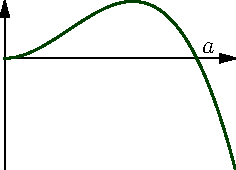
\includegraphics{./Cgd12_1.pdf}
 % Cdg12_1.pdf: 0x0 pixel, 0dpi, 0.00x0.00 cm, bb=
 \caption{Exercice \theenumi}
 \label{fig:Cdg12_1}
\end{figure}

 Soit $m>0$ et $M$ le point de coordonnées $(m,f(m))$. L'équations de la tangente au graphe en ce point est
\begin{displaymath}
 y-f(m) = f'(m)(x-m)
\end{displaymath}
Elle passe par l'origine du repère si et seulement si 
\begin{displaymath}
f(m)=f'(m)m  
\end{displaymath}
Il s'agit de montrer que, sous les hypothèses données, il existe un $m>0$ tel que $f(m)=f'(m)m$.\newline
Considérons la fonction $\varphi$ définie par:
\begin{displaymath}
 \varphi(x)=
\left\lbrace 
\begin{aligned}
 &\frac{f(x)}{x} &\text{ si } x>0 \\
 &0 &\text{ si } x=0
\end{aligned}
\right. 
\end{displaymath}
Par hypothèse, elle est continue en $0$ et dérivable dans $]0,+\infty[$. De plus $\varphi(0)=\varphi(a)=0$, on peut donc lui appliquer le théorème de Rolle entre $0$ et $a$. Il existe un $m>0$ tel que
\begin{displaymath}
 \varphi'(m)=0\Leftrightarrow 
\frac{f'(m)}{m}-\frac{f(m)}{m^2}=0
\Leftrightarrow mf'(m)=f(m)
\end{displaymath}

